\documentclass{article}
\usepackage{amsmath, amssymb}
\usepackage{geometry}
\usepackage{framed}
\geometry{a4paper, margin=1in}
\usepackage{empheq}
\usepackage{xcolor}
\usepackage{booktabs}
% Better formatting for the title
\usepackage[utf8]{inputenc}
\usepackage[T1]{fontenc}
\usepackage{geometry}
\usepackage{fancyhdr}
\usepackage{hyperref}
\usepackage{xcolor}
\usepackage{ragged2e}
\usepackage{amsmath}
\usepackage{graphicx}
\usepackage{bbm}
\usepackage{float}
\usepackage{subcaption}


\geometry{a4paper, margin=1in}
% Header and Footer Setup
\pagestyle{fancy}
\fancyhf{} % Clear default header and footer

% Header
\fancyhead[L]{\textbf{MATH 517 - Statistical Computation and Visualisation}} % Top left above the line
\fancyhead[R]{Assignment 3\textit{}} % Top right above the line
\renewcommand{\headrulewidth}{0.4pt} % Line in the header

% Footer
\fancyfoot[C]{} % Page number at center below the line
\fancyfoot[L]{Leonardo Tonelli} % Professor's name on the left below the line
\fancyfoot[R]{\textbf{Page \thepage}} % Date on the right below the line
\renewcommand{\footrulewidth}{0.4pt} % Line in the footer


\title{}
\author{}
\date{}

\begin{document}
\begin{titlepage}
\centering
    \vspace*{4cm}
    
    % Top horizontal line
    \rule{\textwidth}{1pt}
    \vspace{0.2cm}
    
    {\LARGE\bfseries Assignment 3}
    
    \vspace{0.3cm} % Reduced spacing
    
    {\Large Student: Leonardo Tonelli}
    
    \vspace{0.2cm} % Reduced spacing
    
    {\Large MATH 517 - Statistical Computation and Visualisation}
    
    \vspace{0.3cm} % Reduced spacing
    
    {\large \today}
    
    \vspace{0.2cm}
    
    % Bottom horizontal line
    \rule{\textwidth}{1pt}

    \vspace{10cm}

    {\large \textbf{École Polytechnique Fédérale de Lausanne}} 
    
\end{titlepage}

\section{Theoretical Exercise}

We are given i.i.d. samples $(x_i, y_i), i=1, \ldots n$ from the model:
\[
y_i = m(x_i) + \epsilon_i, \quad i=1, \ldots n
\]
where $x_i \in \mathbb{R}$. The local linear regression estimator at a point $x$ is defined by:
\[
(\hat{\beta}_0(x), \hat{\beta}_1(x)) = \arg\min_{\beta_0,\beta_1 \in \mathbb{R}} \sum_{i=1}^n \left(Y_i - \beta_0 - \beta_1 (X_i - x)\right)^2 K\left(\frac{X_i - x}{h}\right)
\]
where $K$ is a kernel function and $h>0$ is a bandwidth. The fitted value is $\hat{m}(x) = \hat{\beta}_0(x)$.

\subsection{Showing $\hat{m}(x)$ is a Weighted Average}

Let's define the design matrix and weight matrix:
\begin{itemize}
    \item $W_x = \text{diag}\left(K\left(\frac{X_1 - x}{h}\right), \dots, K\left(\frac{X_n - x}{h}\right)\right)$
    \item $X_x = \begin{bmatrix} 1 & X_1 - x \\ \vdots & \vdots \\ 1 & X_n - x \end{bmatrix}$
\end{itemize}

\noindent The weighted least squares solution is:
\[
\hat{\beta}(x) = (X_x^\top W_x X_x)^{-1} X_x^\top W_x Y
\]

\noindent Since $\hat{m}(x) = \hat{\beta}_0(x)$, we extract only the first component by multiplying with $e_1 = (1, 0)^\top$:
\[
\hat{m}(x) = e_1^\top (X_x^\top W_x X_x)^{-1} X_x^\top W_x Y
\].

\noindent Thus, $\hat{m}(x) = \sum_{i=1}^n w_{ni}(x) Y_i$ where:
\[
w_{ni}(x) = e_1^\top (X_x^\top W_x X_x)^{-1} X_x^\top W_x e_i
\]
and $e_i$ is the $i$-th standard basis vector to isolate the ith element of the weight vector. These weights depend only on $\{X_i\}$, $K$, $h$, and $x$, not on $\{Y_i\}$.

\subsection{Explicit Expression for Weights}
To show the equivalence of that expression with the weights just found we need to 
make explicit the vectorized solution for the weight vector and rewrite it in the $S$ notation.\\
Thus, let's compute $X_x^\top W_x X_x$:
\[
X_x^\top W_x X_x = \begin{bmatrix}
\sum_{i=1}^n K\left(\frac{X_i-x}{h}\right) & \sum_{i=1}^n (X_i-x)K\left(\frac{X_i-x}{h}\right) \\
\sum_{i=1}^n (X_i-x)K\left(\frac{X_i-x}{h}\right) & \sum_{i=1}^n (X_i-x)^2 K\left(\frac{X_i-x}{h}\right)
\end{bmatrix}
\]

\noindent Using the notation:
\[
S_{n,k}(x) = \frac{1}{nh}\sum_{i=1}^n (X_i - x)^k K\left(\frac{X_i - x}{h}\right)
\]

\noindent We recognize:
\[
X_x^\top W_x X_x = nh \begin{bmatrix} S_{n,0}(x) & S_{n,1}(x) \\ S_{n,1}(x) & S_{n,2}(x) \end{bmatrix}
\]

\noindent The inverse is:
\[
(X_x^\top W_x X_x)^{-1} = \frac{1}{nh[S_{n,0}(x)S_{n,2}(x) - S_{n,1}^2(x)]} \begin{bmatrix} S_{n,2}(x) & -S_{n,1}(x) \\ -S_{n,1}(x) & S_{n,0}(x) \end{bmatrix}
\]

\noindent Since $\hat{m}(x) = \hat{\beta}_0(x) = e_1^\top \hat{\beta}(x)$ where $e_1 = (1, 0)^\top$, we get:
\[
\hat{m}(x) = \sum_{i=1}^n w_{ni}(x) Y_i
\]

\noindent The weights become:
\[
w_{ni}(x) = \frac{1}{nh[S_{n,0}(x)S_{n,2}(x) - S_{n,1}^2(x)]} \left[S_{n,2}(x) - S_{n,1}(x)(X_i - x)\right] K\left(\frac{X_i - x}{h}\right)
\]

\subsection{Proof That Weights Sum to 1}

We need to show $\sum_{i=1}^n w_{ni}(x) = 1$.

\begin{align*}
\sum_{i=1}^n w_{ni}(x) &= \frac{1}{nh[S_{n,0}(x)S_{n,2}(x) - S_{n,1}^2(x)]} \sum_{i=1}^n \left[S_{n,2}(x) - S_{n,1}(x)(X_i - x)\right] K\left(\frac{X_i - x}{h}\right) \\
&= \frac{1}{nh[S_{n,0}(x)S_{n,2}(x) - S_{n,1}^2(x)]} \left[S_{n,2}(x) \sum_{i=1}^n K\left(\frac{X_i - x}{h}\right) - S_{n,1}(x) \sum_{i=1}^n (X_i - x)K\left(\frac{X_i - x}{h}\right)\right]
\end{align*}

\noindent Using the definitions of $S_{n,k}(x)$:
\begin{align*}
\sum_{i=1}^n K\left(\frac{X_i - x}{h}\right) &= nh \cdot S_{n,0}(x) \\
\sum_{i=1}^n (X_i - x)K\left(\frac{X_i - x}{h}\right) &= nh \cdot S_{n,1}(x)
\end{align*}

\noindent Substituting these expressions:
\begin{align*}
\sum_{i=1}^n w_{ni}(x) &= \frac{S_{n,2}(x)(nh S_{n,0}(x)) - S_{n,1}(x)(nh S_{n,1}(x))}{nh[S_{n,0}(x)S_{n,2}(x) - S_{n,1}^2(x)]} \\
&= \frac{nh[S_{n,0}(x)S_{n,2}(x) - S_{n,1}^2(x)]}{nh[S_{n,0}(x)S_{n,2}(x) - S_{n,1}^2(x)]} \\
&= 1
\end{align*}

\noindent This completes the proof that the weights sum to 1.

\section{Practical Exercise}
\subsection{Simulation Study Setup}
\subsubsection*{Aim of the Study}
This simulation study investigates how the asymptotically optimal bandwidth $h_{AMISE}$ for local linear regression depends on various factors: sample size $n$, block size $N$ used in parameter estimation, and the distribution of covariates $X$ through Beta distribution parameters $(\alpha, \beta)$.
The function to estimate will be referenced multiple times, then we put a figure here displaying it in a plot, for reference:
\begin{figure}[H]
\centering
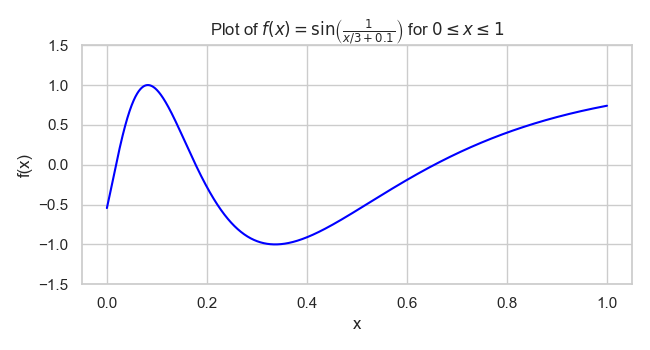
\includegraphics[width=0.6\textwidth]{real_y.png}
\caption{The true regression function $m(x) = \sin\left((x/3 + 0.1)^{-1}\right)$ to be estimated}
\label{fig:y_real}
\end{figure}

\subsubsection*{Simulation Design and Implementation}
The study is implemented in python, and its key components are:

\begin{itemize}
    \item \textbf{Data Generation}:
    \begin{itemize}
        \item Covariates $X$ generated from Beta$(\alpha, \beta)$ distribution
        \item Response $Y = m(X) + \epsilon$ where $m(x) = \sin\left((x/3 + 0.1)^{-1}\right)$ and $\epsilon \sim N(0,1)$
        \item Multiple iterations (5 per configuration) ensure statistical stability
        \item Seeds are managed for reproducibility purposes
    \end{itemize}
    
    \item \textbf{Quantile-based Blocking Implementation}:
    The blocks are not taken with the same length, but based off quantiles of the distribution of our covariates $X$. 
    In this way each block has the same amount of points, facilitating fitting $\hat{m}(x)$ for each block in undersampled examples of our covariates and sparse Beta distribution.
    \begin{itemize}
        \item Partitioned into $N$ blocks using $\texttt{np.quantile(X, np.linspace(0, 1, N+1))}$
        \item Each block contains approximately equal number of observations: $\text{block}_j = [q_{(j-1)/N}, q_{j/N}] \quad \text{for } j=1,\dots,N$
        \item blocks with $<5$ observations skipped to ensure reliable polynomial fitting
    \end{itemize}
    
    \item \textbf{Parameter Estimation Procedure}:
    \begin{itemize}
        \item Polynomial $m_j(x) = \beta_0 + \beta_1x + \beta_2x^2 + \beta_3x^3 + \beta_4x^4$ fitted in each block using sklearn built in functions
        \item Second derivative computed analytically: $m_j''(x) = 2\beta_2 + 6\beta_3x + 12\beta_4x^2$
        \item $\hat{\theta}_{22} = \frac{1}{n}\sum_{i=1}^n \sum_{j=1}^N [m_j''(X_i)]^2 \mathbf{1}_{\{X_i \in \text{block}_j\}}$
        \item $\hat{\sigma}^2 = \frac{1}{n-5N}\sum_{i=1}^n \sum_{j=1}^N [Y_i - m_j(X_i)]^2 \mathbf{1}_{\{X_i \in \text{block}_j\}}$
    \end{itemize}
    
    \item \textbf{Bandwidth Calculation}:
    \[
    h_{AMISE} = n^{-1/5} \left( \frac{35 \hat{\sigma}^2 \cdot |\text{supp}(X)|}{\hat{\theta}_{22}} \right)^{1/5}
    \]
    and since $X \sim Beta$:
    $$
    |\text{supp}(X)| = 1 \quad \text{(for Beta distribution on [0,1])}$$

    \item \textbf{Simulations}: 
    The simulations are run in \textbf{three} different data collection loops. In the first one, the bandwidth $h_{AMISE}$
    is collected for different pairs of Beta parameters and for different sample sizes leaving $N$ as fixed at the optimal value computed with the $C_p$ criterion.
    The second loop instead (used to study the effect of blocks number $N$), compute the optimal bandwidth for varying sample size $n$ and varying Beta distributions. 
    Lastly, a simulation is run to evaluate the relationship between optimal $N$ and $n$, this compute the $N$ optimal for varying sizes of the samples and different beta distributions, without recomputing the bandwidth $h_{AMISE}$.
    In all three cases, the computations is repeated 5 times with different data samples, to ensure robustness of results and complete visualization.
\end{itemize}

\paragraph{Optimization Procedure}
When they are studied the effect of the Beta distribution parameters and the sample size n, it is chosen a fixed optimal block size $N$ using Mallow's $C_p$ criterion, as suggested in the text of the exercise.
Then it is chosen a block number $N$ such that the following criterion is minimized:
\[
C_p(N) = \frac{RSS(N)}{RSS(N_{\max})/(n-5N_{\max})} - (n - 10N)
\]
where $N_{\max} = \min(n/20, 10)$ ensures sufficient data per block. The implementation also includes robust error handling for edge cases.

\subsection{Results and Discussion}

\paragraph{Effect of Sample Size ($n$)}

The plot in Figure~\ref{fig:sample_size} clearly demonstrates the theoretical relationship \( h_{\text{AMISE}} \propto n^{-1/5} \). As the sample size increases from 250 to 2000, the \textbf{optimal bandwidth decreases} gradually for all Beta distributions. 
However, the decrease occurs at a slower rate for the Beta(5,2) distribution. This can be explained by the behavior of the true function \( m(x) \), shown in Figure~\ref{fig:y_real}, which is relatively simple and linear on the right side of its support. 
Because the Beta(5,2) distribution draws most covariates \( X \) from this region, the sampled data presents a function that appears simpler. Consequently, the optimal bandwidth does not require the same degree of refinement to capture complex local features, 
which explains its slower rate of decrease as the sample size grows.

\begin{figure}[H]
\centering
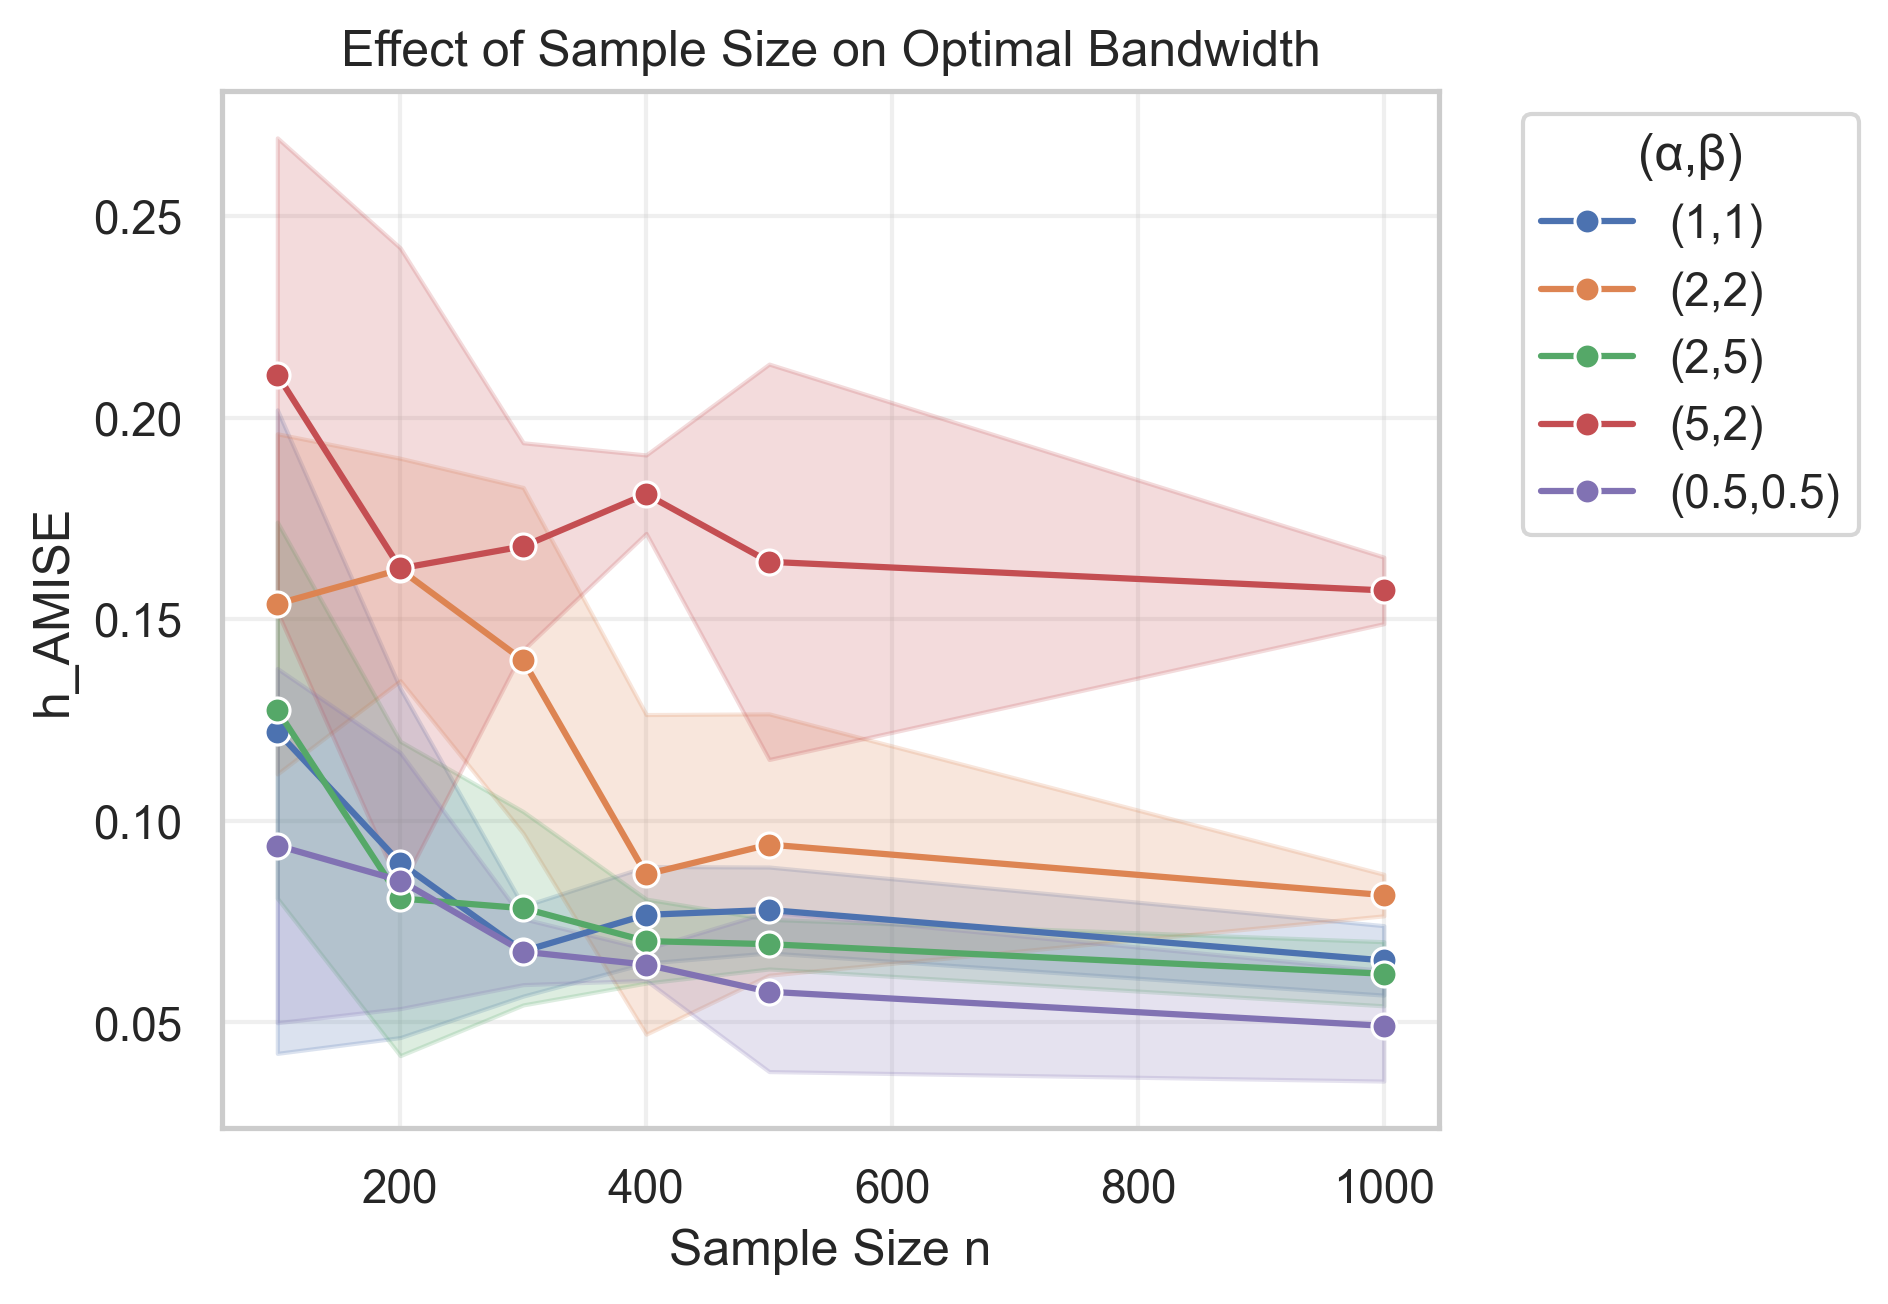
\includegraphics[width=0.5\textwidth]{plot1_sample_size_effect.png}
\caption{Impact of sample size $n$ on optimal bandwidth $h_{AMISE}$}
\label{fig:sample_size}
\end{figure}


\paragraph{Behavior of $h_{AMISE}$ as $N$ Grows} The graph in Figure~\ref{fig:block_N} reveals a clear \textbf{inverse relationship} between the optimal bandwidth $h_{\text{AMISE}}$ and the block size $N$. For all covariate distributions studied,
the bandwidth decreases gradually as the number of blocks \textbf{increases}.

\begin{figure}[H]
\centering
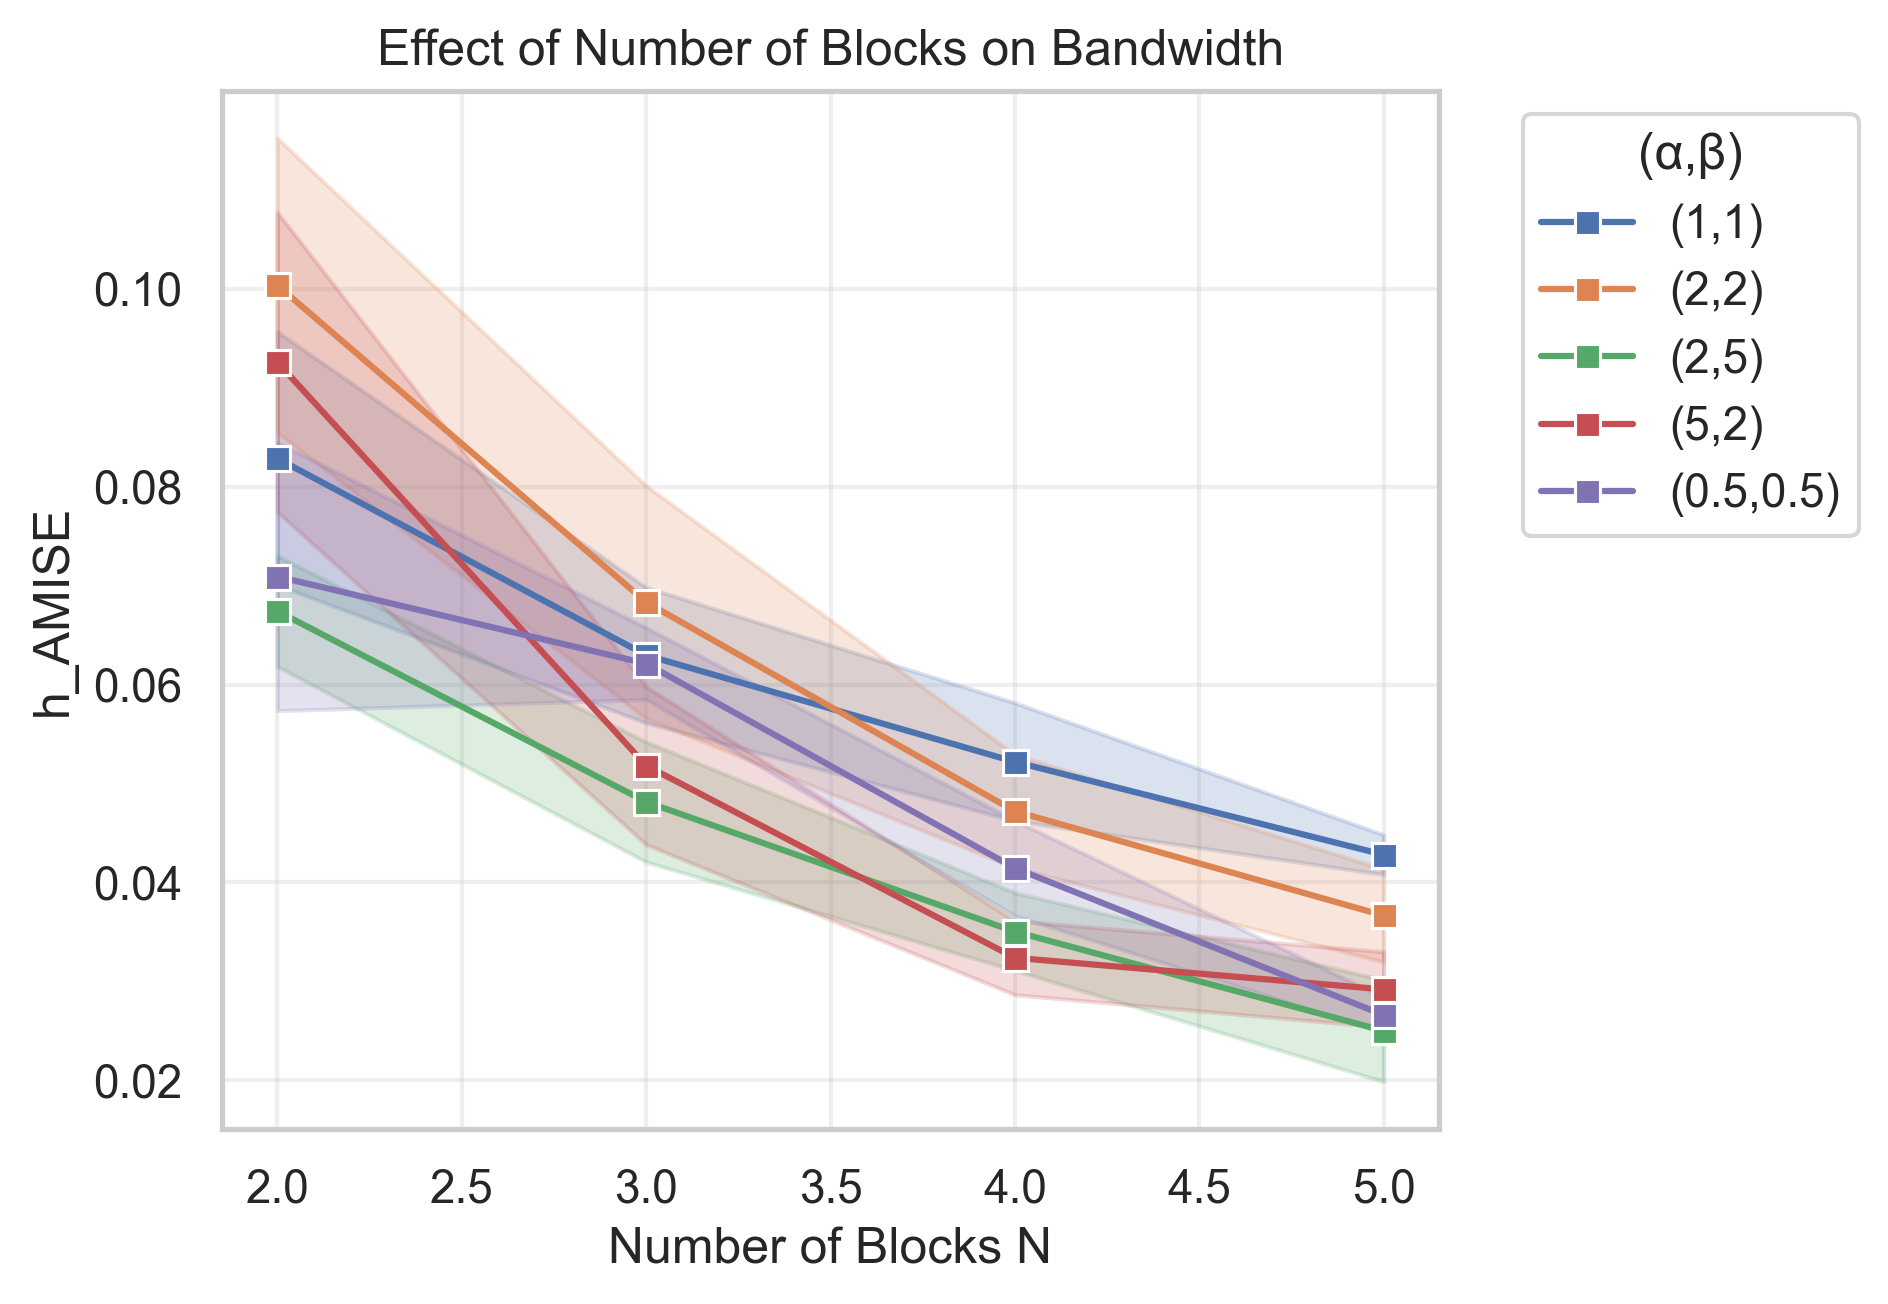
\includegraphics[width=0.5\textwidth]{plot2_block_size_effect.png}
\caption{Impact of block numbers $N$ on optimal bandwidth $h_{AMISE}$}
\label{fig:block_N}
\end{figure}

To investigate this relationship we plot the variations of our estimates for $\hat{\theta}_{22}$ and $\hat{\sigma}^2$ when the number of blocks
increases from 2 to 5. From Figures \ref{fig:sigma}, \ref{fig:theta} we can see that the estimates for the variance remains in the interval $[0.9,1.10]$ without a clear pattern. On the other hand, $\hat{\theta}_{22}$
rises at increasing blocks number $N$, for every sample size $n$. Notice how the plot is in log scale, to highlight the difference between the values.


\begin{figure}[H]
\centering
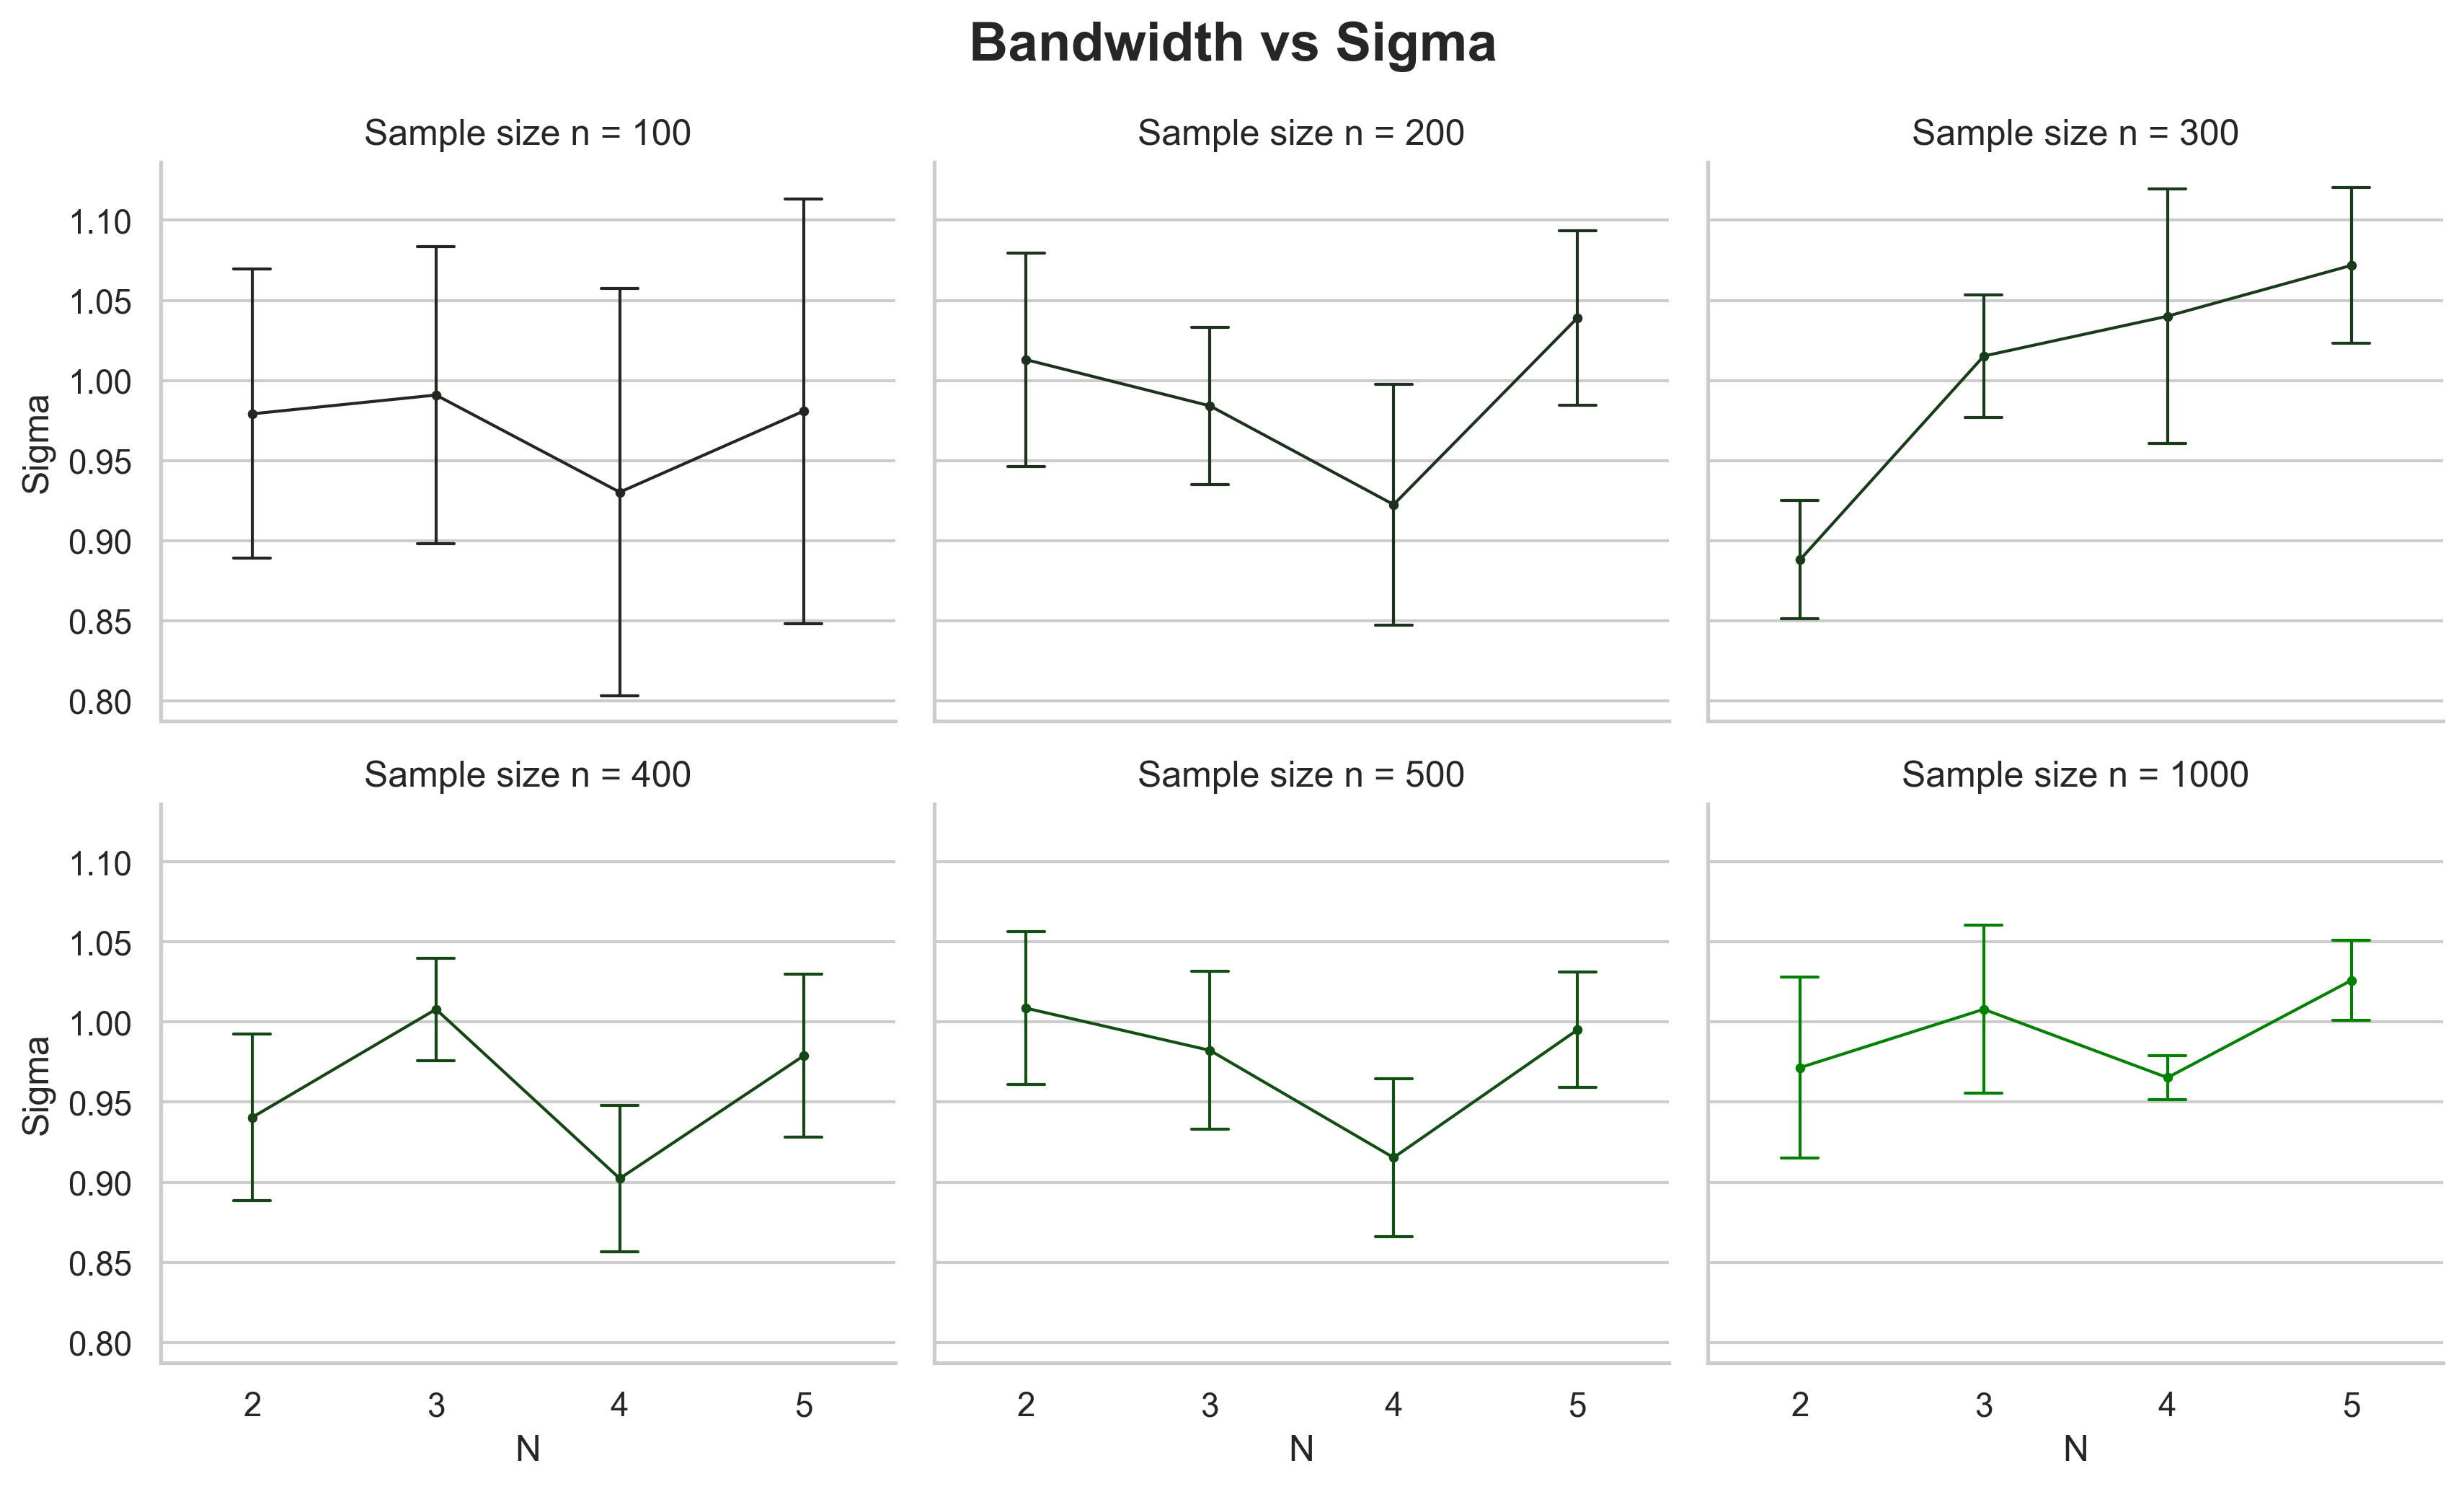
\includegraphics[width=0.5\textwidth]{N_vs_sigma.png}
\caption{Impact of block numbers $N$ on $\hat{\sigma}^2$}
\label{fig:sigma}
\end{figure}

\begin{figure}[H]
\centering
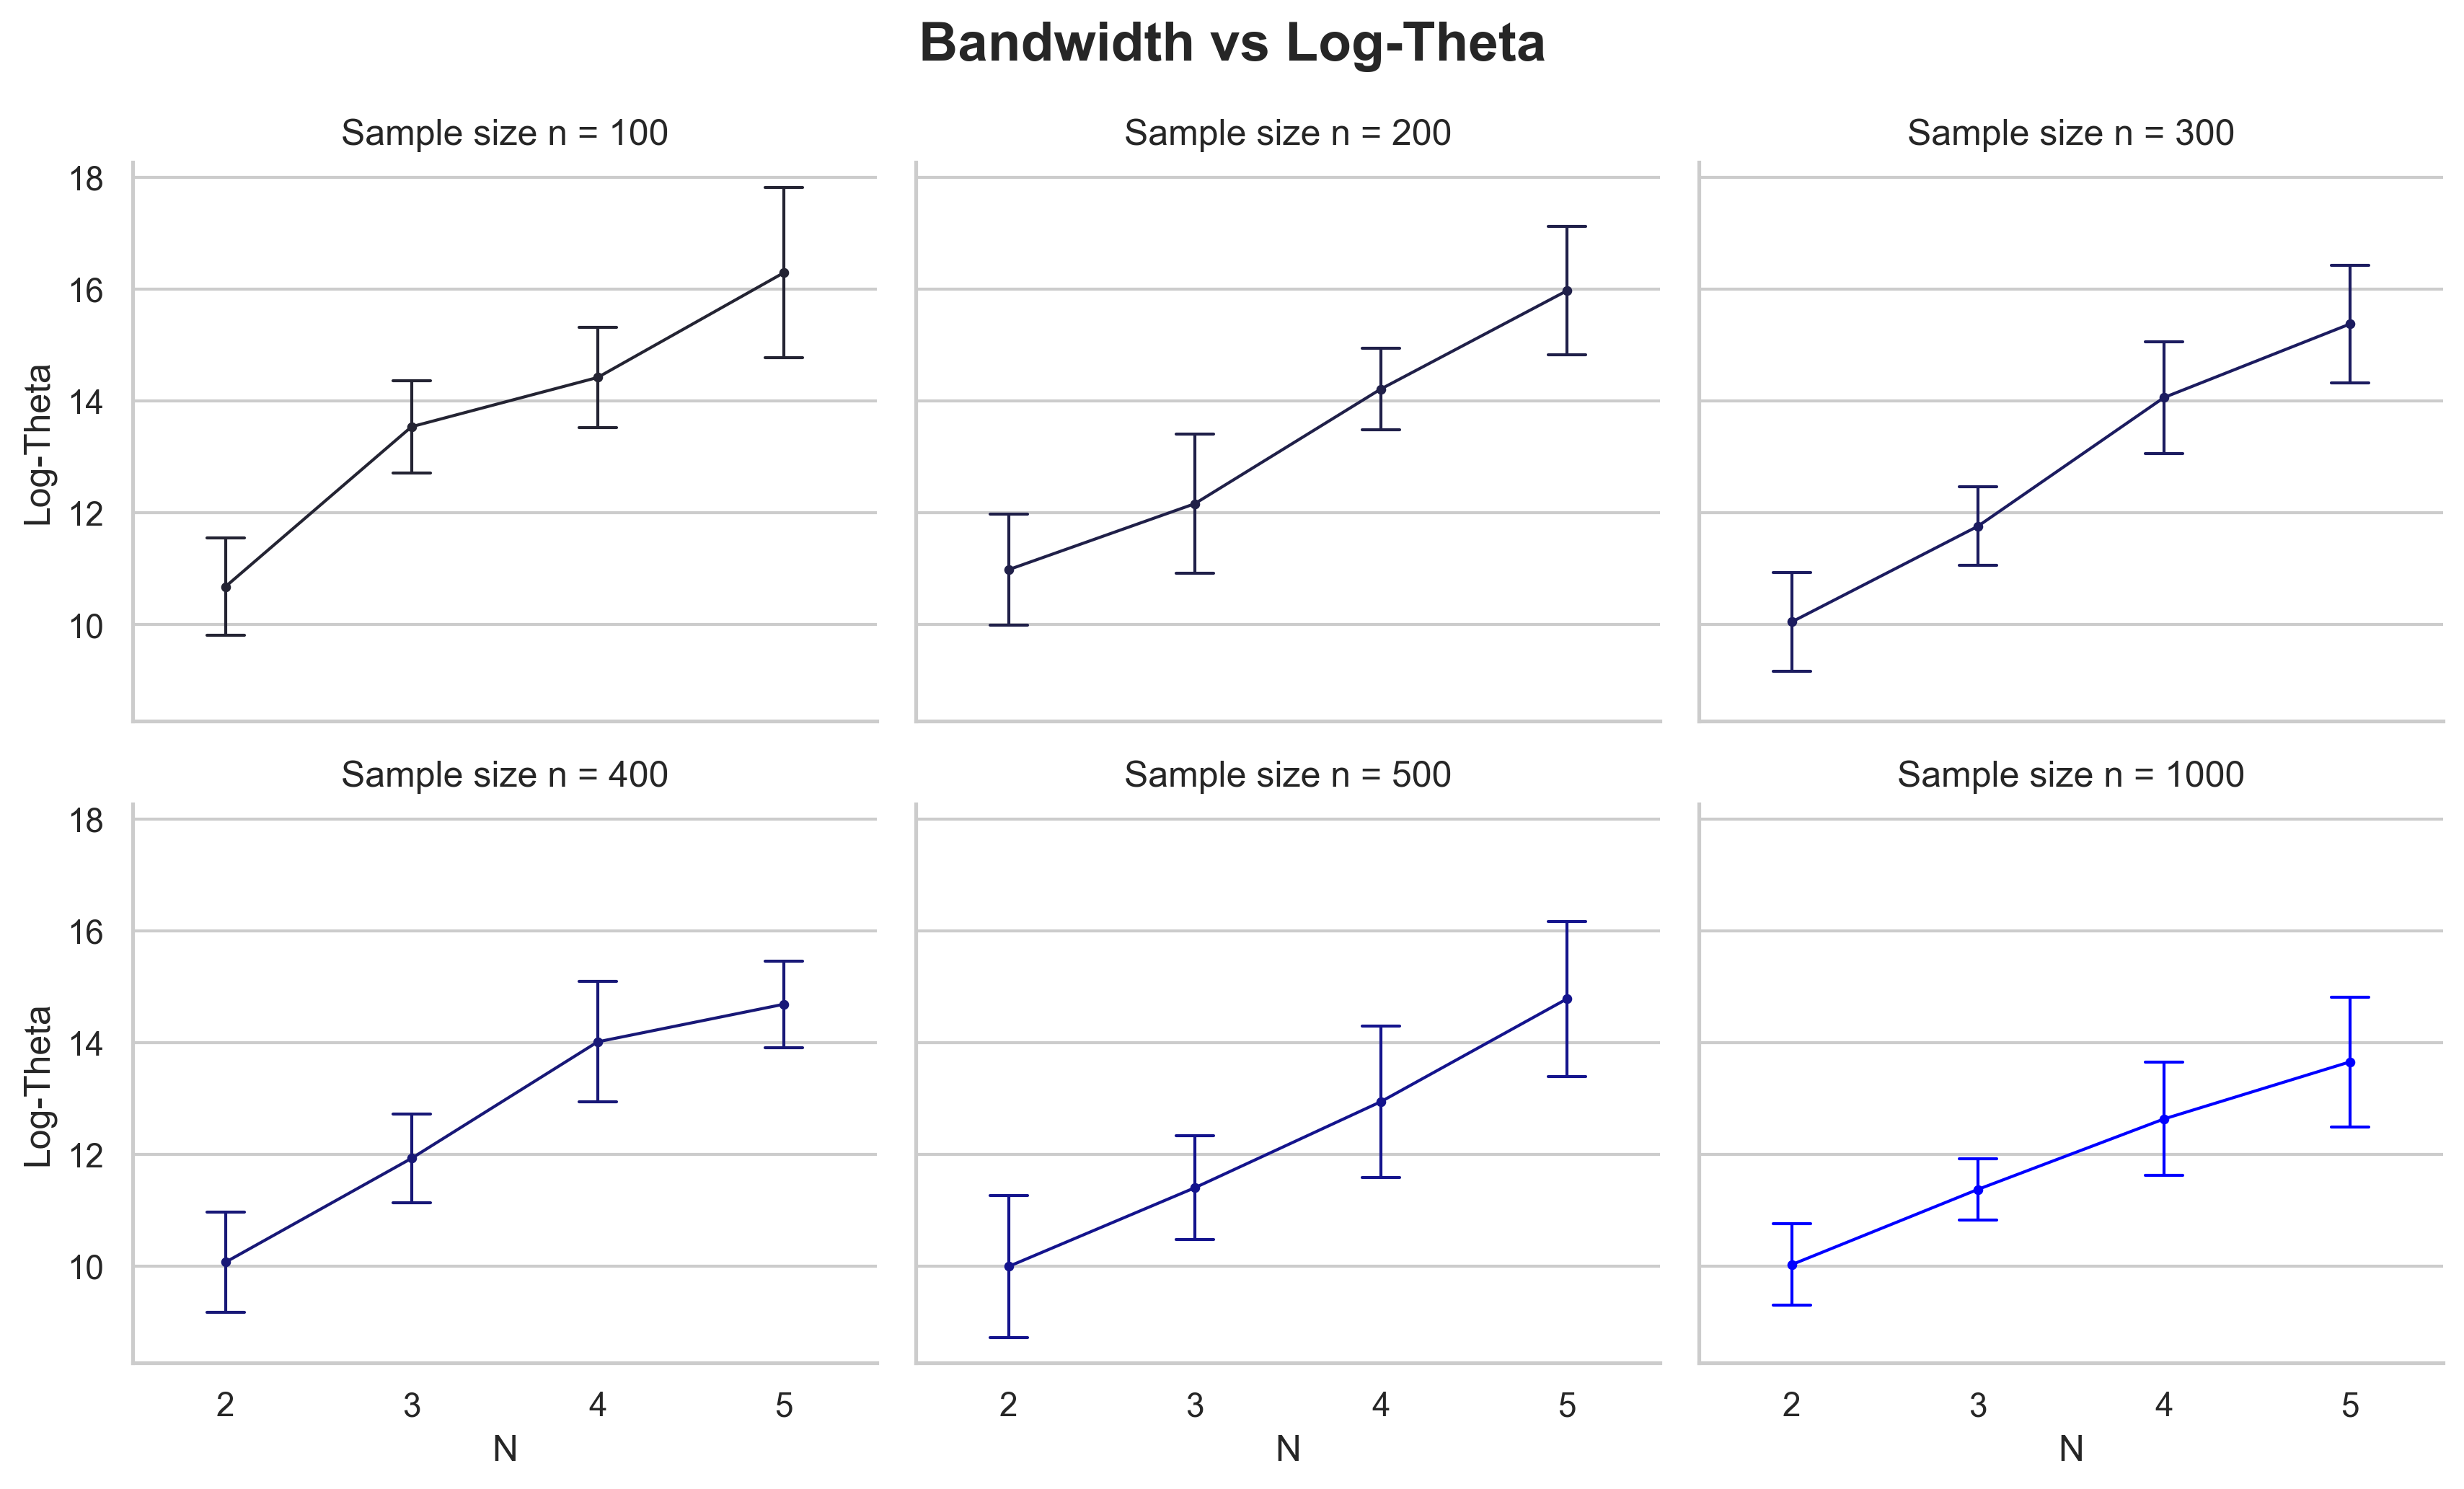
\includegraphics[width=0.5\textwidth]{N_vs_theta.png}
\caption{Impact of block numbers $N$ on $\hat{\theta}_{22}$}
\label{fig:theta}
\end{figure}

This is because as $N$ increases, the data is partitioned into smaller, more localized subsets. 
Within these smaller blocks, the local quartic polynomial $\hat{m}_j$ can more flexibly adapt 
to local variations and curvature, leading to fitted functions $\hat{m}_j(x)$ that are more 
"wiggly" or have larger second derivatives within their respective blocks. Consequently, when 
these local second derivatives $\hat{m}''_j(X_i)$ are aggregated across the entire dataset to 
compute $\hat{\theta}_{22}$, the result is a larger estimated curvature. Since the formula for 
$h_{AMISE}$ is inversely proportional to the fifth root of $\theta_{22}$ ($h_{AMISE} \propto 
(\theta_{22})^{-1/5}$), the observed increase in $\hat{\theta}_{22}$ directly drives the 
decrease in the optimal bandwidth.

\paragraph{Should $N$ depend on $n$? Why?}
Intuitively, $N$ should depend on $n$ because the number of blocks governs a fundamental 
trade-off. With too few blocks ($N$ too small for a given $n$), the local polynomial models 
are too rigid and may fail to capture the underlying function's genuine local curvature, 
leading to high bias. Conversely, with too many blocks ($N$ too large), each block contains 
too few data points to reliably fit a quartic polynomial, causing the estimates to become 
unstable and noisy—a clear case of overfitting that increases variance. Therefore, the 
optimal $N$ must scale with $n$ to navigate this bias-variance trade-off; more data allows 
for a finer partition of the support to reduce bias, but only if each resulting block still 
has sufficient data to control variance.

To test this idea, we examined how the optimal number of blocks $N$ (using Mallow criterion) changes with sample size $n$.
Figure~\ref{fig:Nvsn} shows this relationship. We see a gradual increase in optimal $N$ as $n$ 
grows, suggesting that more data allows for finer data partitioning. With small samples, using 
few blocks prevents overfitting. With larger samples, we can use more blocks to better capture 
local patterns. However, this growth eventually levels off because the true function's 
complexity is limited—using too many blocks eventually provides no further benefit.

\begin{figure}[H]
\centering
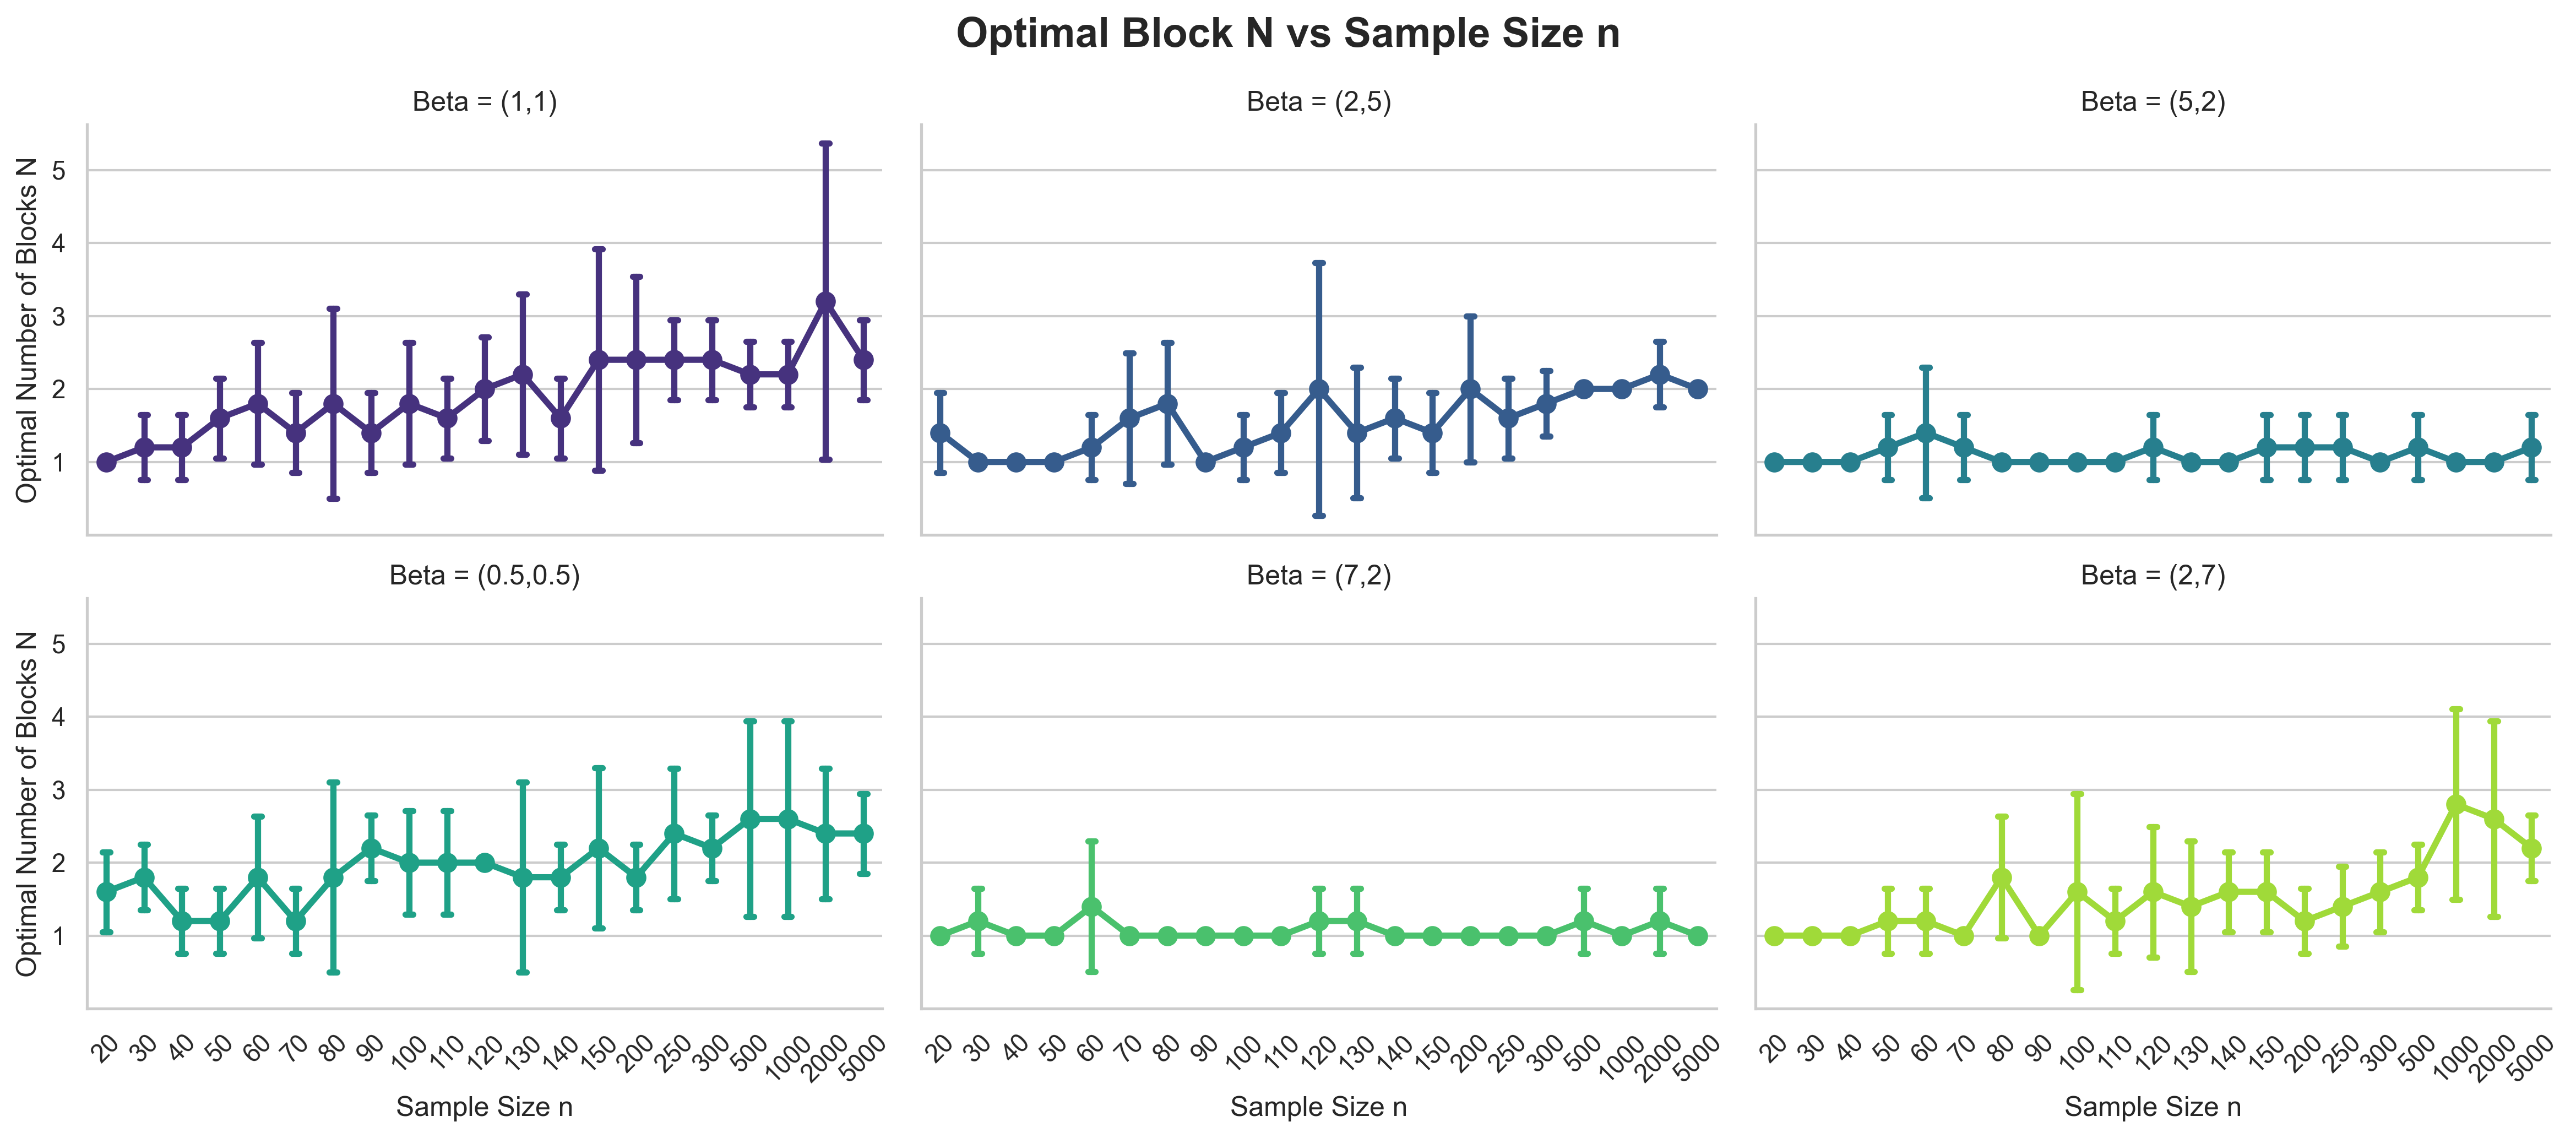
\includegraphics[width=0.7\textwidth]{plot4_block_vs_n.png}
\caption{Relationship between optimal $N$ and sample size $n$}
\label{fig:Nvsn}
\end{figure}

Interestingly, for left-skewed Beta distributions, the optimal number of blocks stays at 
$N^* = 1$ regardless of sample size. This occurs because these distributions sample mostly 
from the right side of the function's domain, where $m(x)$ behaves simply and linearly. 
Here, a single global polynomial fits well, making multiple blocks unnecessary. This shows 
that the relationship between $n$ and $N$ depends strongly on where the data is concentrated 
and the local complexity of the function in those regions.


\paragraph{Bandwidth $h_{\text{AMISE}}$ with different sampling distributions}
Figure~\ref{fig:beta} displays the average optimal bandwidth $h_{\text{AMISE}}$ (over 5 iterations) for different sample sizes $n$, where the block size $N$ is selected by minimizing Mallow's $C_p$. 
An interesting pattern emerges for the Beta(2,5) and Beta(5,2) distributions, where the optimal bandwidth for one is consistently much smaller than the other. As the accompanying density plots illustrate (Figures \ref{a}, \ref{b}), 
these two distributions are \textbf{skewed} in opposite directions. Consequently, the covariate sampling they produce features regions with a \textbf{substantial difference in the concentration} of data points.
\begin{figure}[H]
    \centering
    \begin{subfigure}{0.3\textwidth}
        \centering
        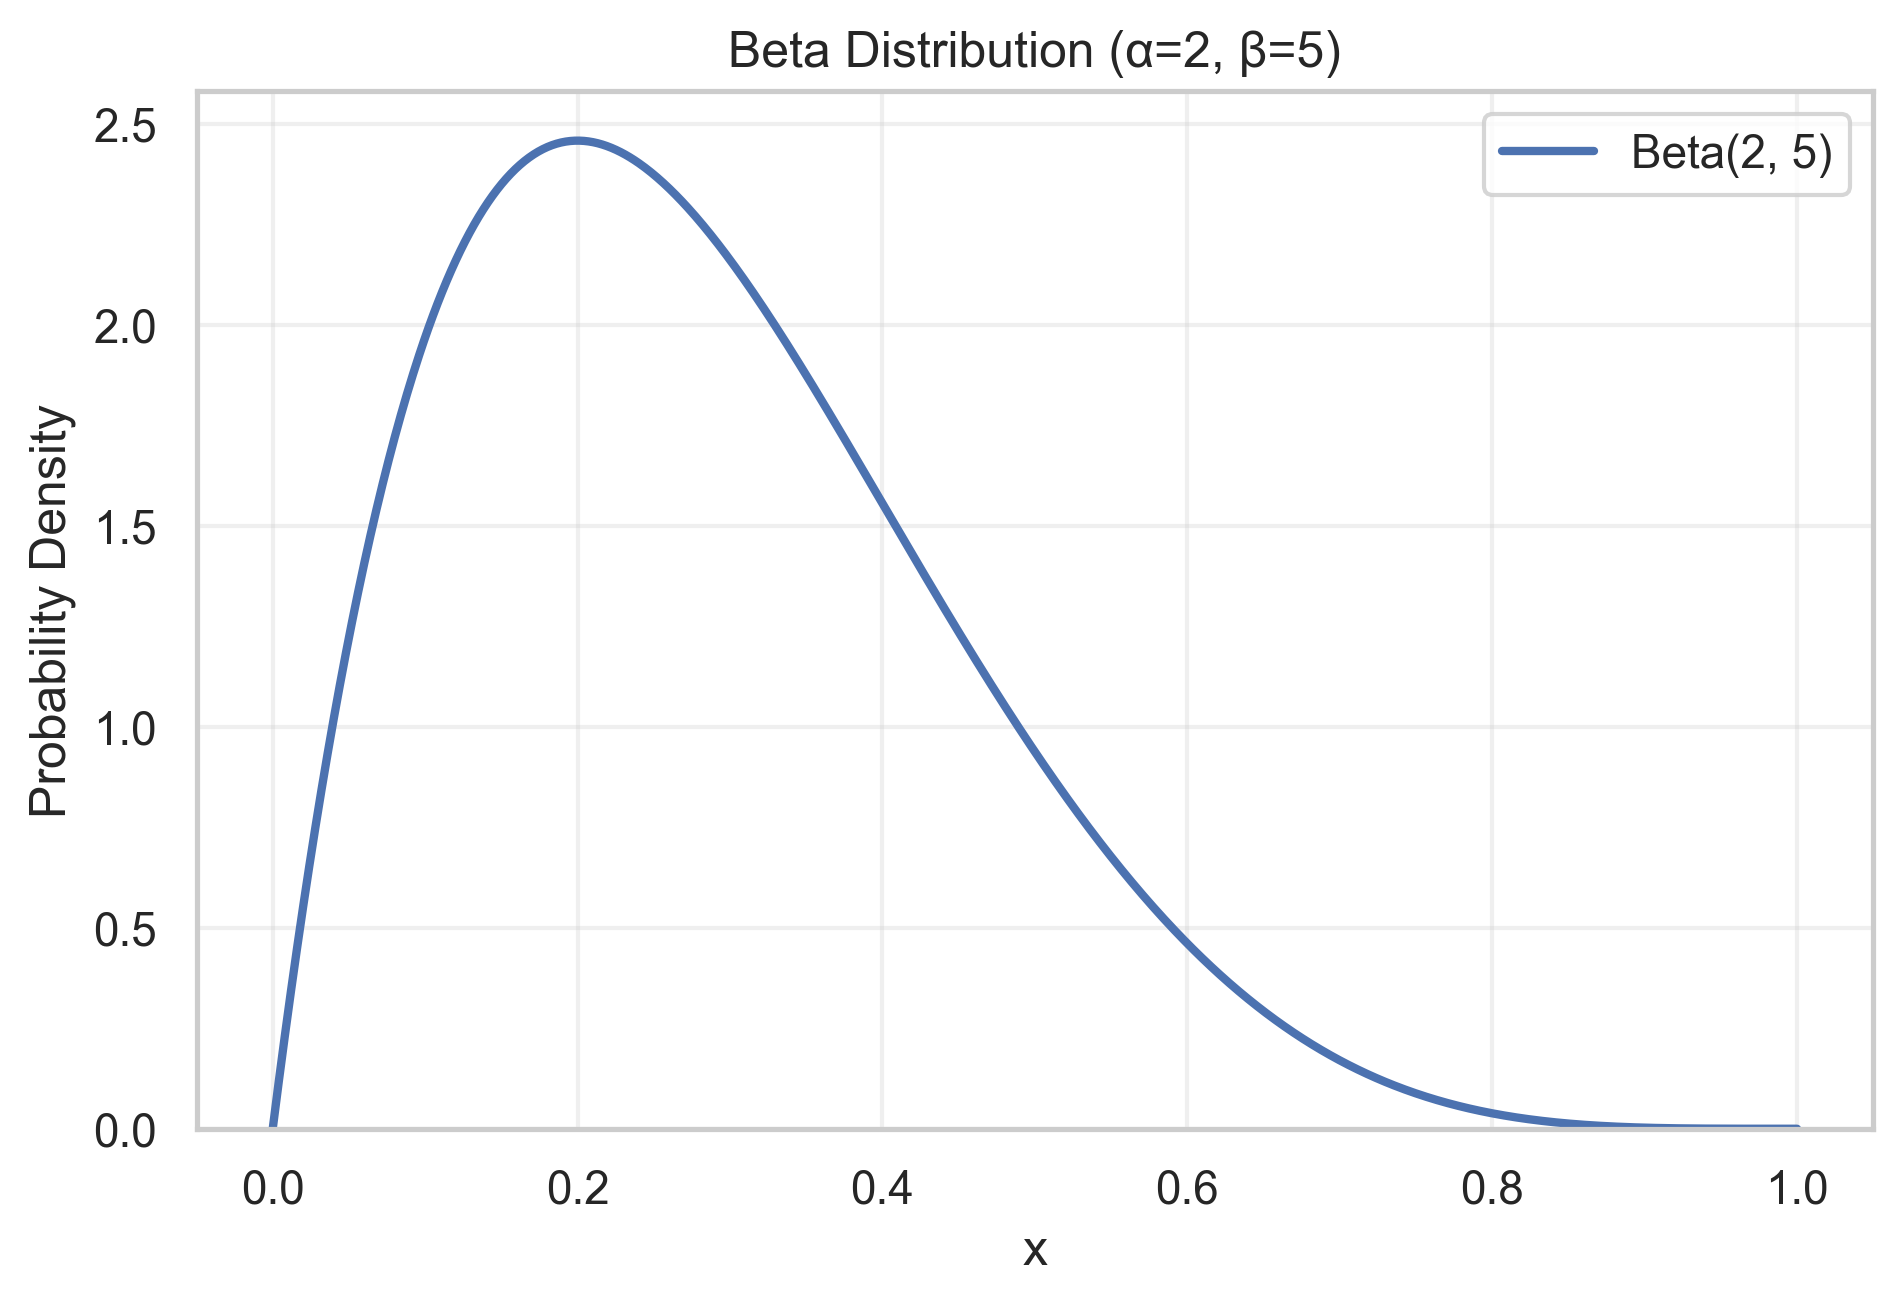
\includegraphics[width=\textwidth]{beta_distribution1.png}
        \caption{$Beta(2, 5)$}
        \label{a}
    \end{subfigure}
    \hspace{0.05\textwidth} % Reduced space between images
    \begin{subfigure}{0.3\textwidth}
        \centering
        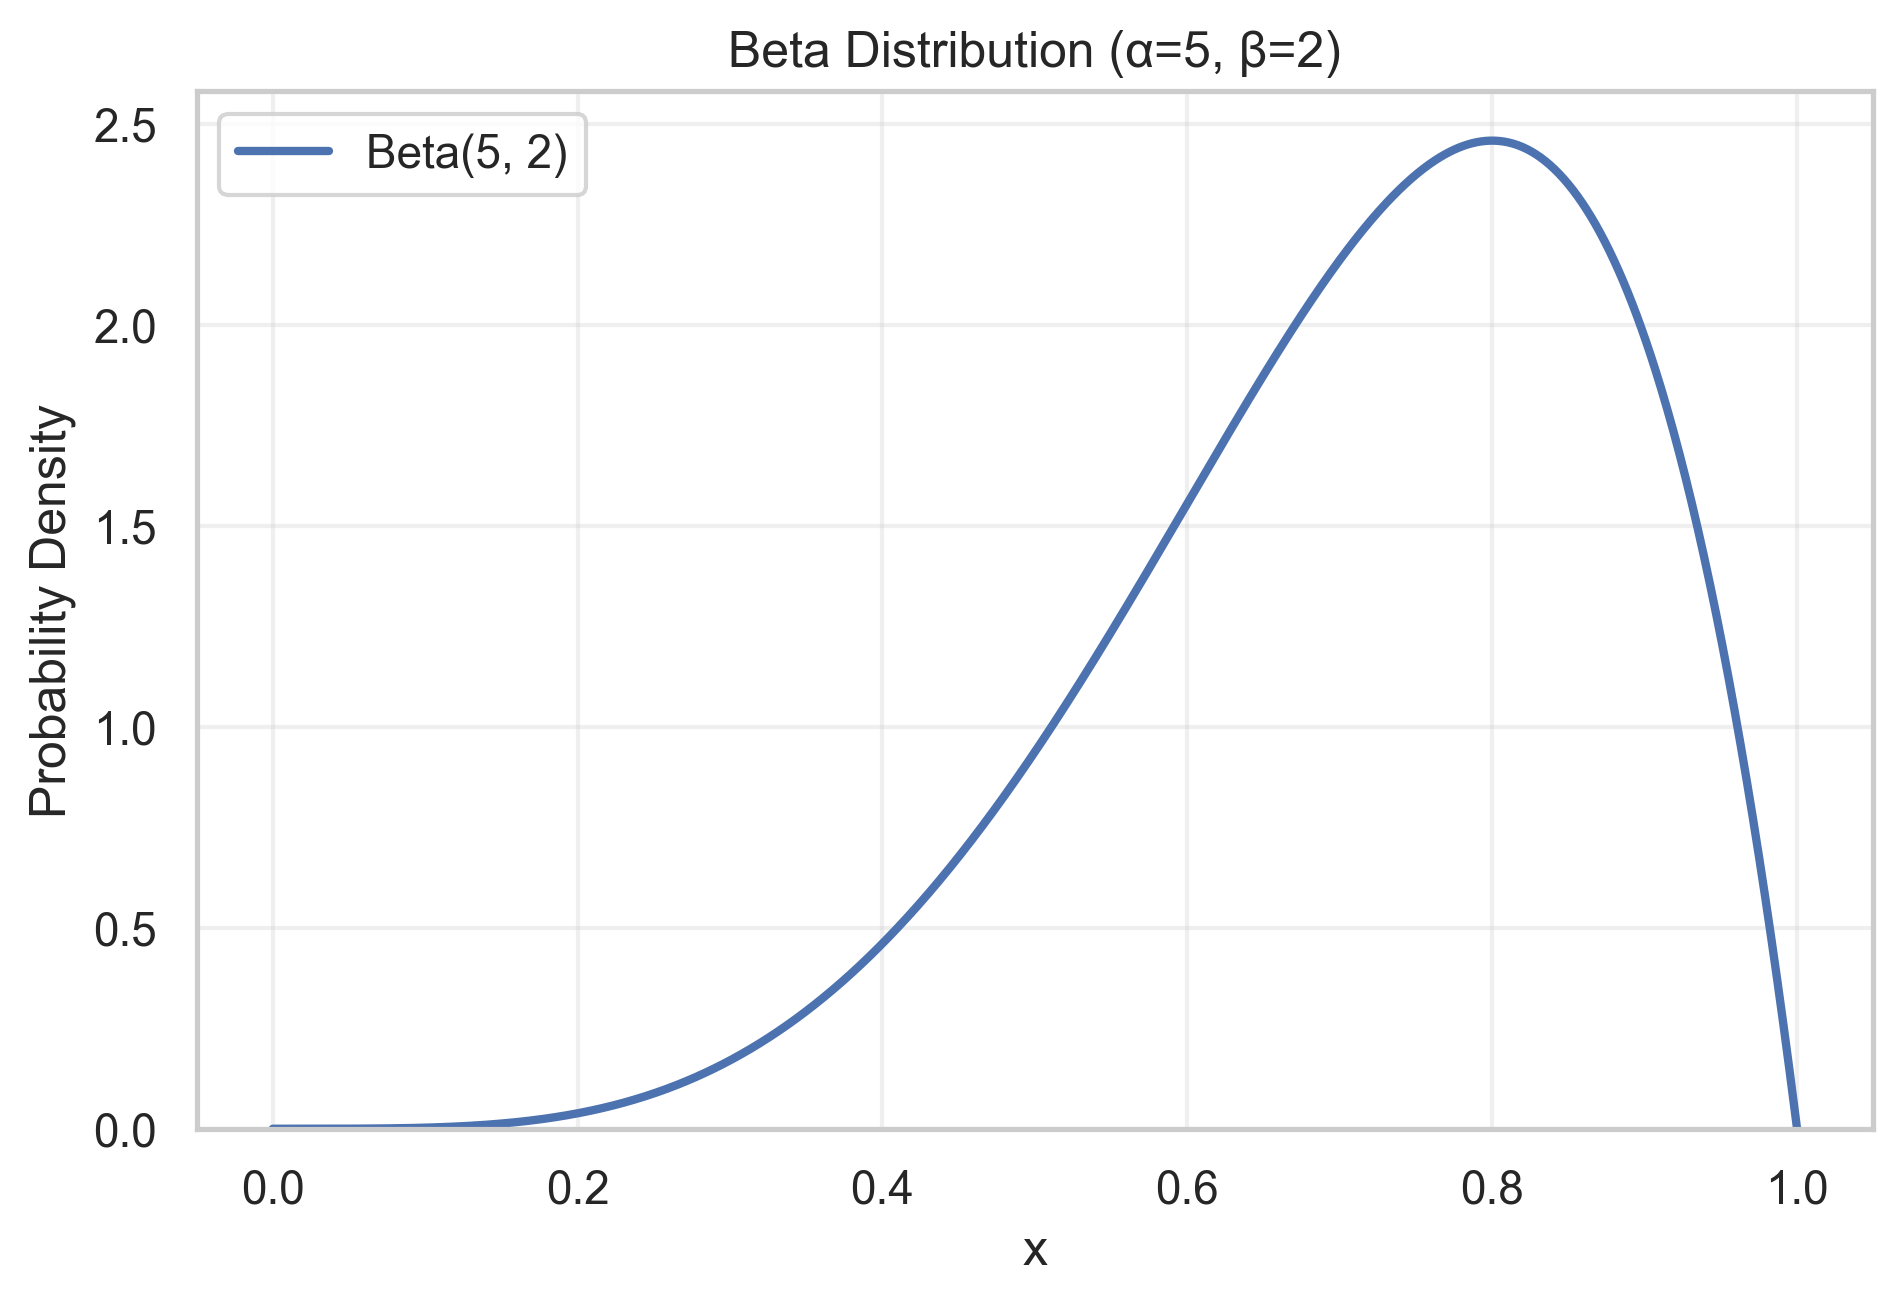
\includegraphics[width=\textwidth]{beta_distribution2.png}
        \caption{ $Beta(5, 2)$}
        \label{b}
    \end{subfigure}
    \label{fig:beta_comparison}
\end{figure}

The optimal bandwidth \( h_{\text{AMISE}} \) is much lower for the right-skewed distribution (Beta(5,2)) than for the left-skewed one (Beta(2,5)). 
This phenomenon could be explained by the \textbf{geometry} of the true function \( m(x) \) in Figure~\ref{fig:y_real}. The function exhibits higher curvature on the left side of its domain compared to the more linear behavior on the right.
When the covariate sample is concentrated on the right (Beta(5,2)), the local fits of \( \hat{m} \) primarily capture this simple, linear relationship, which is reflected in a smaller optimal bandwidth. This results in an estimator 
that is simpler but may be less accurate globally. Conversely, when samples are concentrated on the left (Beta(2,5)), the optimal bandwidth must be larger to accommodate the complex local curvature of the underlying function, leading 
to a final estimate that is more likely to be wiggly and overfit to the specific sample.

\begin{figure}[H]
\centering
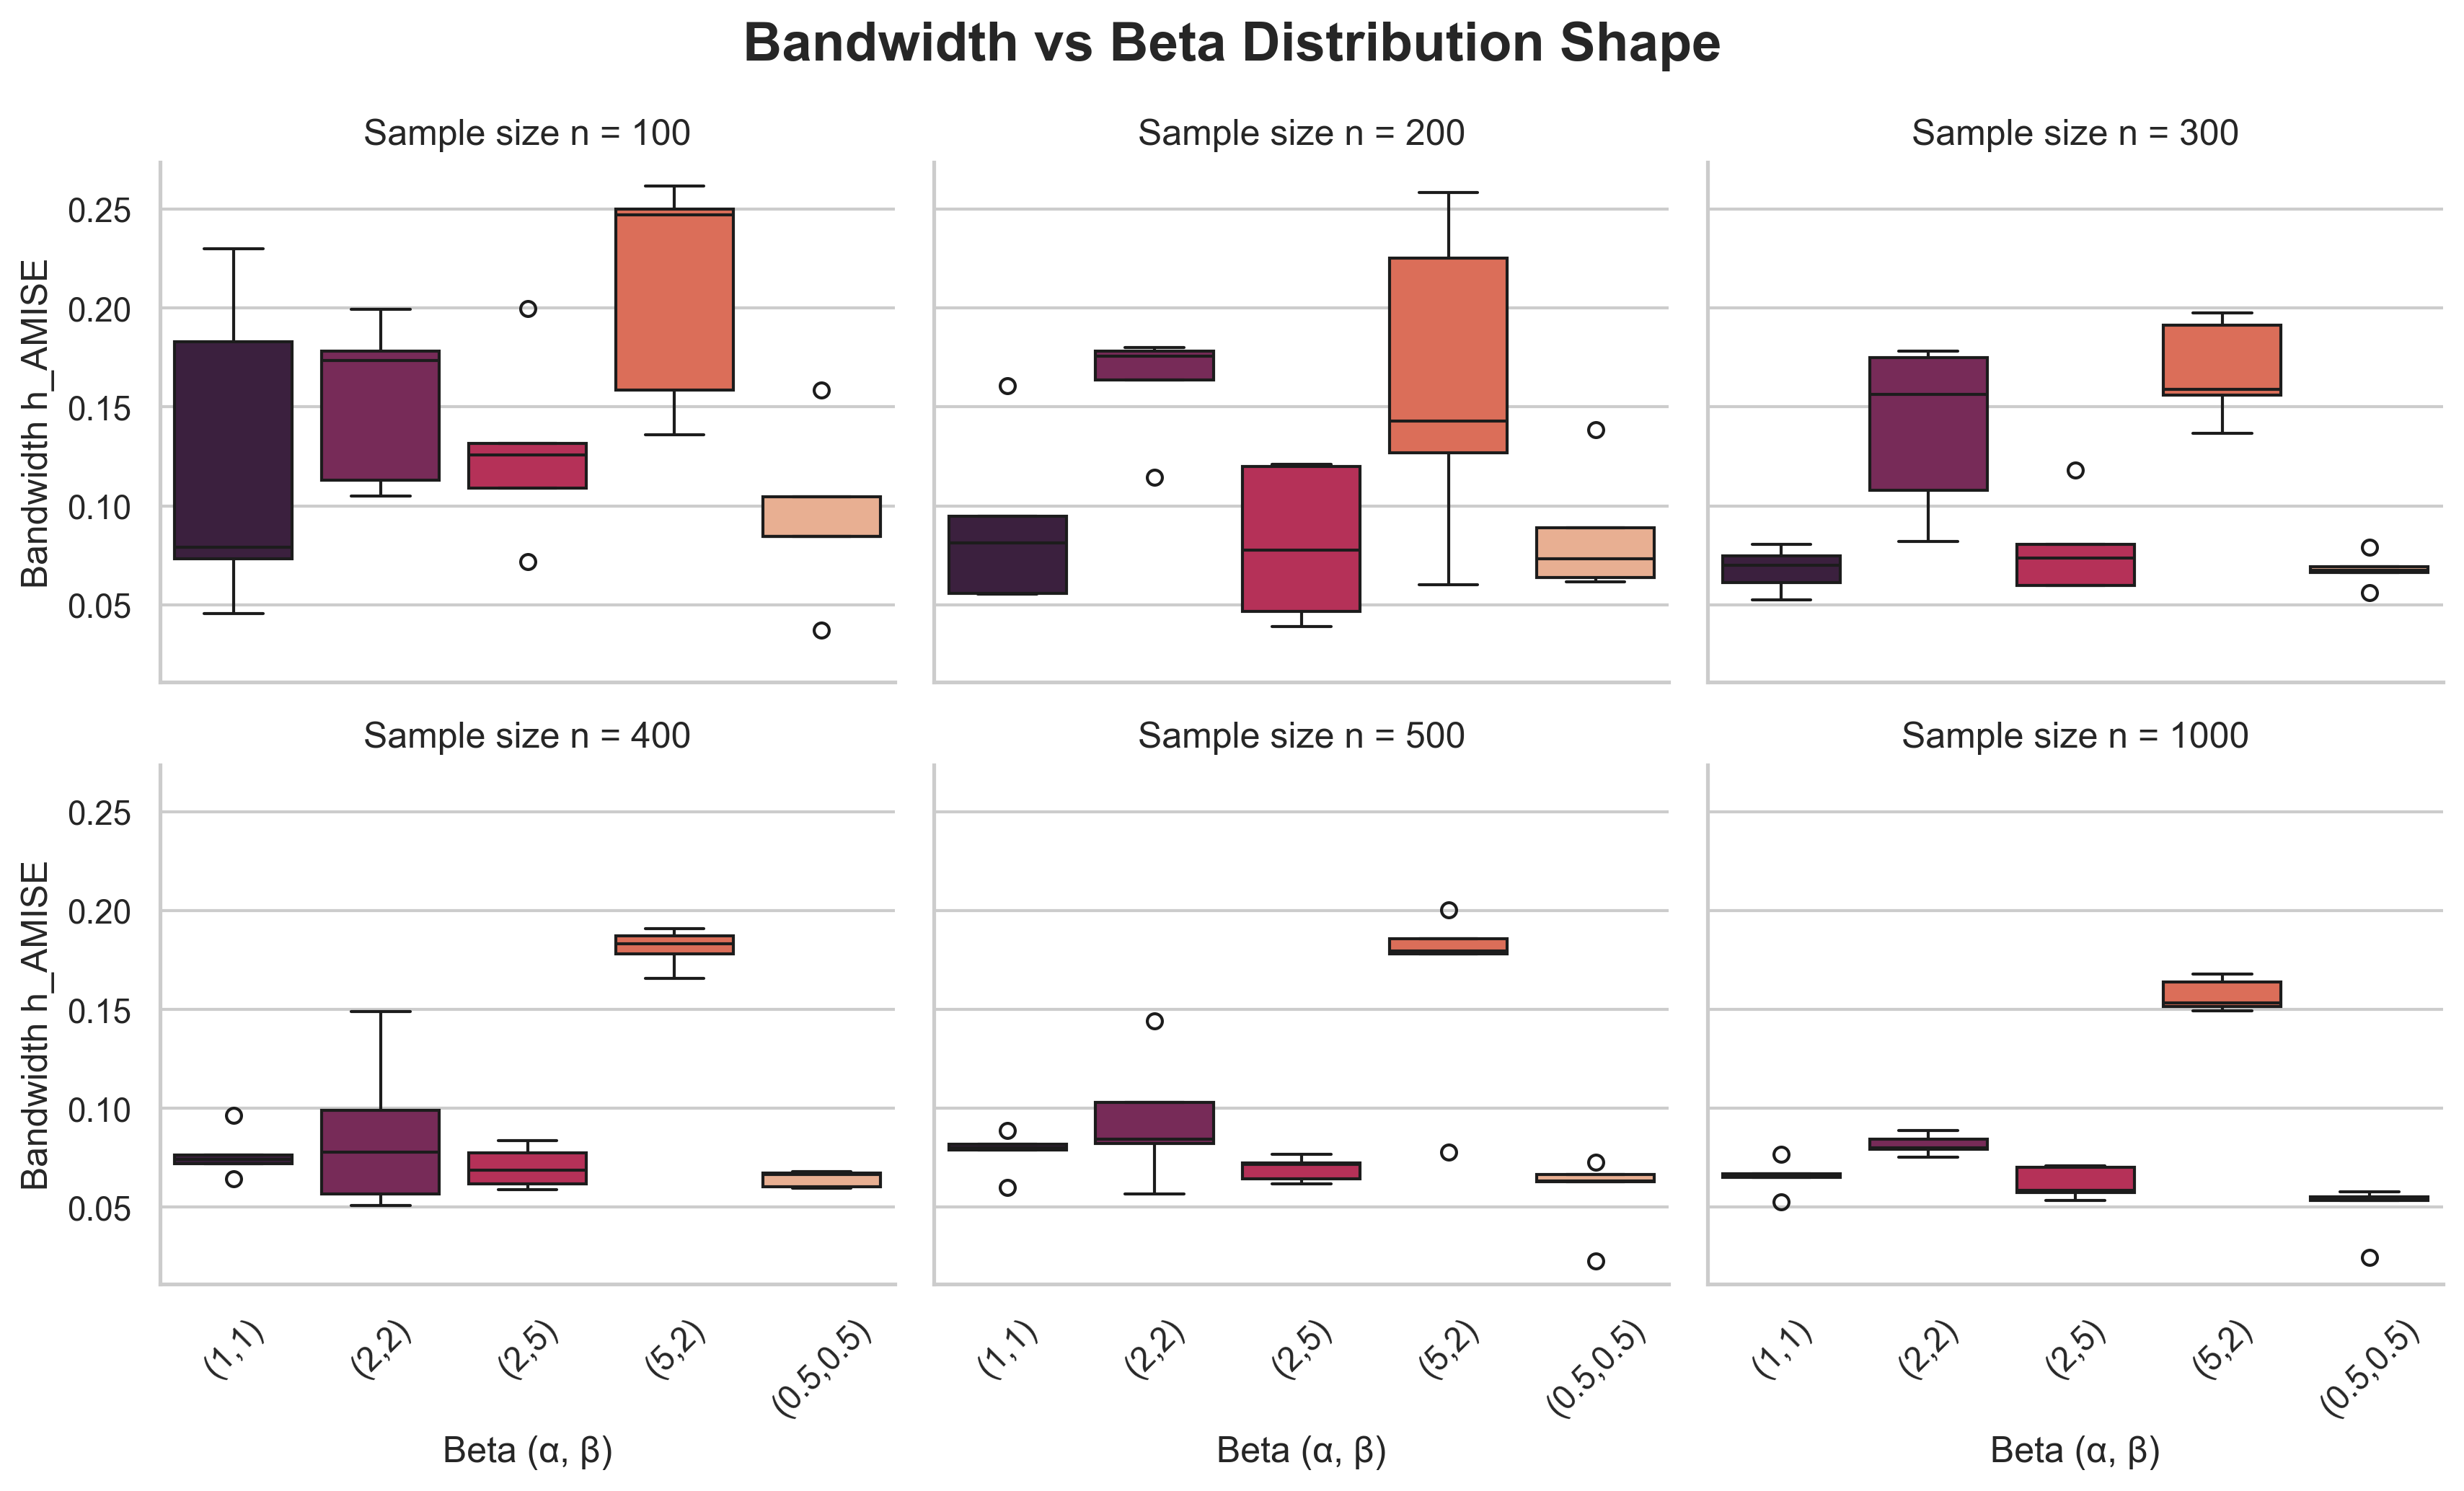
\includegraphics[width=0.70\textwidth]{plot3_beta_vs_bandwidth.png}
\caption{Impact of Beta distribution on optimal bandwidth $h_{AMISE}$}
\label{fig:beta}
\end{figure}


\subsubsection*{Conclusion}
This simulation study confirms that the optimal bandwidth $h_{\text{AMISE}}$ is \textbf{sensitive} to the sample size $n$, the block parameter $N$, and the covariate distribution. 
The results validate the theoretical $n^{-1/5}$ scaling and demonstrate that the data distribution's shape directly influences bandwidth selection by highlighting regions of differing functional complexity. 
Furthermore, the block size $N$ should scale with $n$ to optimize the bias-variance trade-off, but this relationship is bounded by the inherent complexity of the underlying function.
\end{document}